\documentclass{article}
\usepackage[margin=1in]{geometry}
\usepackage{graphicx}
\usepackage{caption}
\usepackage{subcaption}
\usepackage{float}
\usepackage{amsmath}
\usepackage{booktabs}

\setcounter{secnumdepth}{0}

\title{Memory masking vs overwriting in procedural categorization}
\author{}
\date{}

\begin{document}

\maketitle

\section{Authors}
Matthew J. Crossley\textsuperscript{1,2,3*}\\
Jack Mair\textsuperscript{1}\\
David M. Kaplan\textsuperscript{1,2,3}\\\\
\textbf{1} School of Psychological Sciences, Macquarie University, Sydney, Australia \\
\textbf{2} Performance and Expertise Research Centre, Macquarie University, Sydney, Australia \\
\textbf{3} Macquarie Minds and Intelligences Initiative, Macquarie University, Sydney, Australia

\section{Abstract}
Behaviors acquired through procedural learning systems such
as athletic skills (e.g., a cricket bat swing) are highly
robust and notoriously resistant to change, even when they
become contaminated by maladaptive habits (e.g., an
inefficient follow-through). Identifying effective methods
for modifying such procedural knowledge is therefore a major
challenge. Previous work suggested that feedback contingency
(i.e., the degree to which behavior causes outcomes) is a
critical factor determining whether procedural knowledge can
be modified. Specifically, Crossley, Ashby, and Maddox
(2013) reported that an intervention combining random and
veridical feedback appeared to erase recently acquired
procedural category knowledge. In the present study, we
directly tested this claim. Across two experiments, we
examined whether feedback manipulations lead to true
unlearning of stimulus–response associations or instead
merely mask their behavioral expression. We used
decision-bound modeling and Bayesian estimation of
reacquisition rates to provide clear evidence that mixed
random–veridical feedback does not erase procedural
knowledge. Instead, it merely masks expression.  Learning
rapidly re-emerged when participants were verbally cued that
valid feedback had resumed. These findings necessitate a
substantial revision of existing models of procedural
category learning. They also have important implications for
approaches to changing procedural skills more broadly.

\section{Introduction}
Habitual behavior has become increasingly prevalent in the
modern environment, where devices and social media platforms
are intentionally designed to promote repeated use. A
growing body of evidence links such habits to negative
outcomes, including attentional fragmentation, reduced
productivity, and heightened risks for anxiety and
depression (REFS).  Beyond individual consequences, the
large-scale adoption of digital habits has been argued to
shape patterns of public discourse, social cohesion, and
even political polarization (REFS). These observations
underscore the broader societal costs of technologically
mediated habits.  Clarifying how such behaviors are
instantiated in the brain, and how they can be disrupted or
regulated, represents a pressing challenge for contemporary
basic and applied research.

A major source of habitual behavior likely lies in the
neural mechanisms supporting operant stimulus-response (SR)
learning. In the animal learning literature, especially in
rodent models, behavior is often characterized as either
goal-directed to habitual. Goal-directed actions are
sensitive to the agent's current goals and motivational
states, enabling flexible adaptation to changing
environmental contingencies. In contrast, habitual behaviors
are rigid, triggered directly by environmental cues, and
often persist even when the associated reward is devalued.
For example, a rat may continue pressing a lever for food
despite being sated, much like a human may continue
scrolling through social media absent any specific goal or
gratification.

In the human cognitive literature, this distinction between
goal-directed and habitual behavior closely parallels the
division between declarative and procedural learning and
memory systems. Declarative memory supports flexible,
hypothesis-driven reasoning and explicit knowledge, while
procedural memory underlies behaviors learned through
reinforcement of repeated experience, typically with little
cognitive effort or conscious awareness. This division is
particularly well studied in the domain of category
learning, where different category structures are thought to
preferentially engage different memory systems.

In recent work, we reported an intervention that appeared to
induce true overwriting of procedural category knowledge.
Participants who had previously acquired a category
structure through procedural learning no longer showed
evidence of this knowledge following the intervention,
suggesting that the learned associations had been erased.
However, rather than eliminating the procedural memory, the
intervention it is possible that the intervention may merely
have masked its behavioral expression. On this account, the
underlying SR mappings remain intact but lie dormant and may
reemerge under appropriate conditions.

In the present study, we directly test this possibility. We
provide clear evidence that the intervention does not result
in unlearning of procedural category knowledge. Instead, it
masks the expression of that knowledge, which remains
accessible under suitable retrieval conditions. These
findings have important implications for how we understand,
measure, and intervene on habit-like behaviors across
domains.

\section{Methods}

\subsection{Experiments and conditions}
The study consisted of two experiments, each comprising
three phases: Learn, Intervention, and Test. Participants
were randomly assigned to one of two between-subject
conditions: \textit{Relearn} or \textit{New Learn}. The
Learn and Test phases were identical across experiments and
conditions. During the Learn phase, participants were
trained on a category structure designed to promote
procedural learning. In the Test phase, they were assessed
either on the same category structure (Relearn) or on a new
one (New Learn). The critical manipulation occurred during
the Intervention phase. In Experiment~1, participants
received fully random feedback, whereas in Experiment~2,
feedback was a mixture of random and veridical.

This design closely follows our previous work, which showed
that fully random feedback does not produce masking or
unlearning of procedural category knowledge, whereas mixed
feedback can induce such effects. To distinguish between
unlearning and masking, we presented the following on-screen
message just before the first trial of the Test phase:

\begin{quote}
Over the last many trials the feedback you received was
random. This was an important part of the experiment. From
now on, the feedback will again be valid. Please keep trying
to categorize correctly. Press the Y key to proceed.
\end{quote}

If mixed feedback causes unlearning, participants should be
unable to reacquire their previously learned procedural
knowledge, and performance in the Test phase should not
exceed that of the Learn phase. By contrast, if mixed
feedback only masks prior learning, participants should be
able to use the instructions to re-express their procedural
knowledge, leading to performance in the Test phase that is
comparable to or better than at the end of the Learn phase.

Experiment~1, in which the intervention was fully random
feedback, served as a control condition to replicate our
previous findings that such feedback does not produce
unlearning. This step was important because the present
study used slightly different stimuli and category
structures from our earlier work.

\subsection{Stimuli and categories}
The stimuli were circular sine-wave gratings that varied in
spatial frequency and orientation.  The coordinates of all
stimuli were generated by first sampling points in polar
coordinates and then converting them into Cartesian
coordinates.  Specifically, radius values $r$ were sampled
from a uniform distribution on the interval $[0, 1]$, and
angle values $\theta$ were sampled uniformly from the
interval $[0, 2\pi]$.  These polar coordinates $(r, \theta)$
were then transformed into Cartesian coordinates $(x, y)$
using the equations $x = r \cos(\theta)$ and $y =
r\sin(\theta)$. This resulted in a set of $(x, y)$
coordinates uniformly distributed within a circle of radius
1 and centered at the origin. Next, $(x,y)$ coordinates were
transformed from a circular uniform distribution to an
elliptical uniform distribution with horizontal major axis
by multiplying the $x$ values by 124.02 and the $y$ values
by 28.44. For the Test phase in the New Learning conditions,
the resulting coordinates were rotated by 45 degrees and
translated by $(40, 60)$ for half the stimuli and by $(60,
40)$ for the other half. The resulting stimulus
distributions are shown in Figure~\ref{fig_cat}.

\begin{figure}[H]
    \centering
    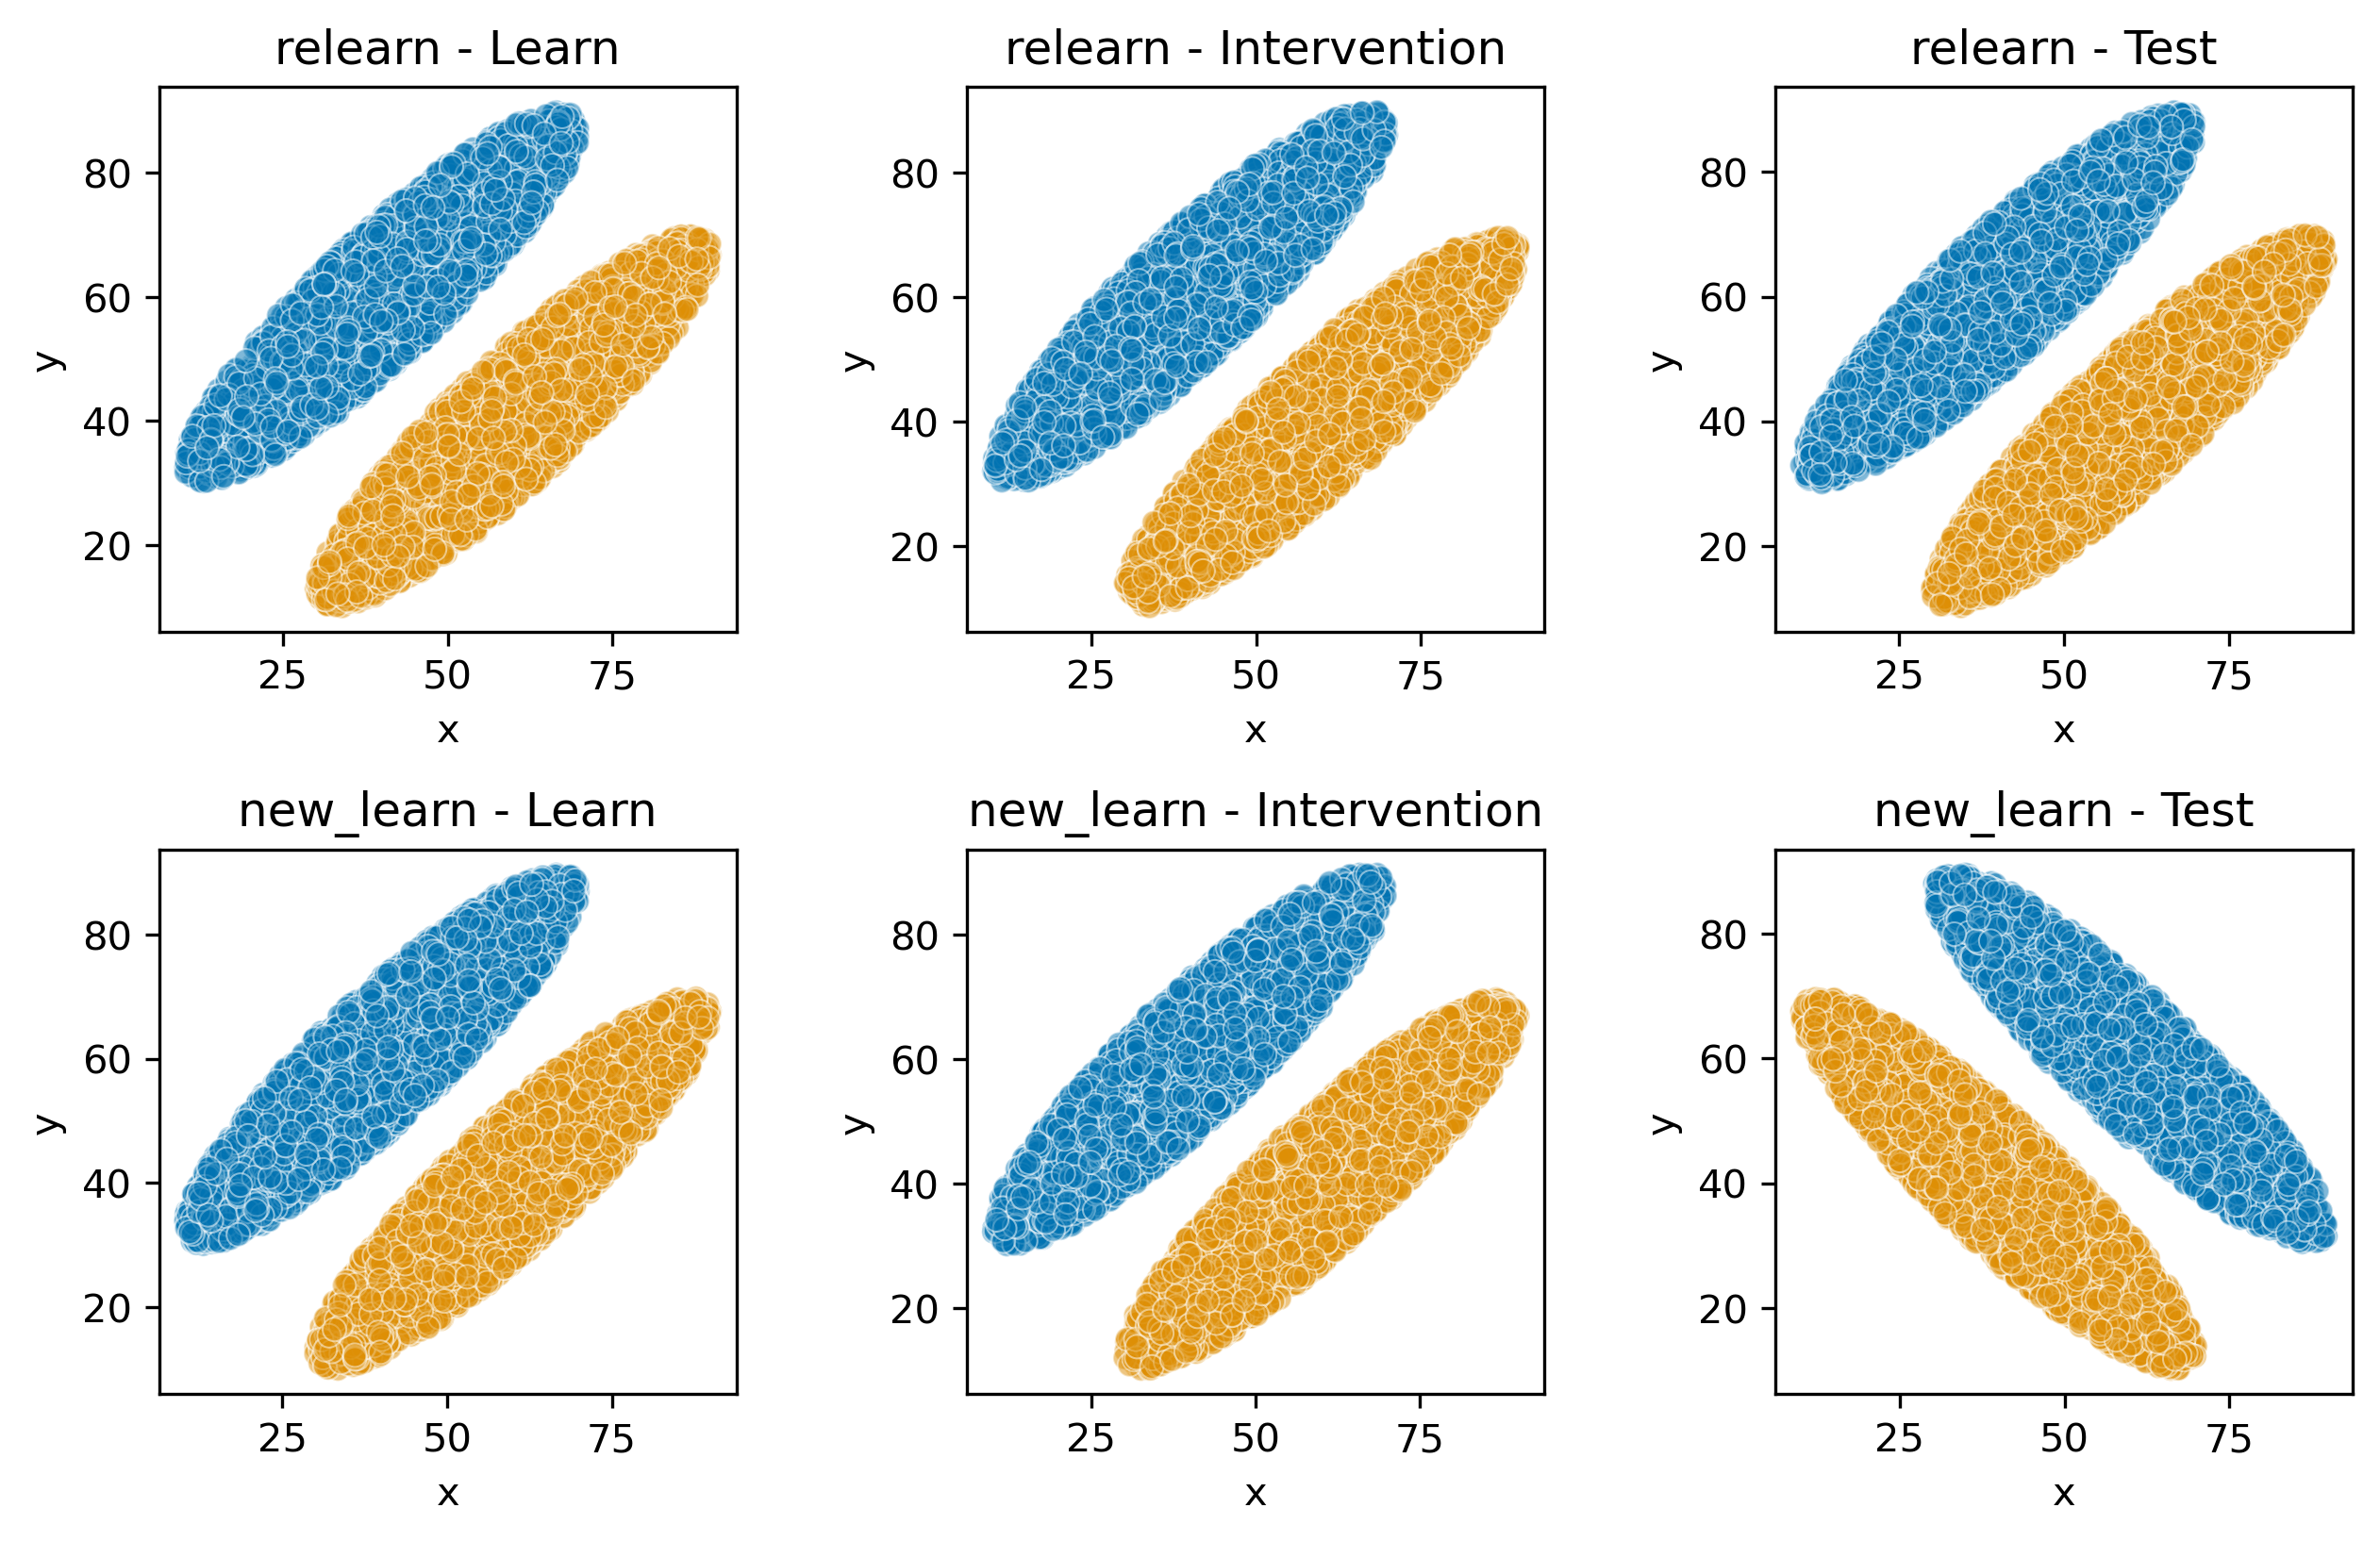
\includegraphics[width=\textwidth]{../figures/fig_cat_struct.png}
    \caption{}
    \label{fig_cat}
\end{figure}

Category learning can be described within a multiple-systems
framework that distinguishes between declarative and
procedural mechanisms \cite{ashby1998differentiating,
ashby2017multiple}.  Declarative category learning relies on
explicit reasoning and hypothesis testing. Rule-based (RB)
tasks are commonly used to study this system, as they
typically require participants to apply simple, verbally
describable rules (e.g., if orientation exceeds a threshold,
choose Category A; otherwise, choose Category B)

Procedural category learning, by contrast, depends on the
gradual formation of stimulus--response associations
acquired through reinforcement of direct experience.
Information-integration (II) tasks are typically used to
study this system. These tasks require learners to combine
information across multiple stimulus dimensions in a way
that cannot be easily verbalized. Unlike RB learning, where
performance often improves suddenly following discovery of
the correct rule, II learning is characterized by
incremental trial-by-trial improvements
\cite{maddox2004dissociating, ashby2011}.

Evidence that RB tasks are primarily learned with
declarative systems and II learning is primarily learned
with procedural systems comes from behavioral, neuroimaging,
and patient studies (for reviews, see REF). In the present
study, we employ II categories because they specifically
engage procedural mechanisms, thereby providing a window
into the stimulus--response processes that underlie broader
habitual behaviors.

\subsection{Procedure}
Participants provided informed consent and were given an
optional demographic questionnaire to complete. Participants
were instructed that their task was to categorize circular
sine-wave gratings on the basis of their spatial frequency
and orientation, and that each category was equally likely.
Each participant completed a single session consisting of
900 trials. Each phase (Learn, Intervention, Test) consisted
of 300 trials. On each trial, participants viewed a fixation
cross (1000 ms), followed by a response-terminated stimulus,
and then feedback (1000 ms).  Responses were given via the
``d'', and ``k'' keys.  Feedback following correct responses
was a green circle that appeared around the stimulus, and
feedback following incorrect responses was a red circle. See
Figure~\ref{fig_example_trials} an illustration of example
trials.

\subsection{Participants}
A total of 40 participants were recruited for Experiment 1
(32 female, 8 male), with ages ranging from 18 to 32 years
(M = 20.33, SD = 2.61). An additional 40 participants took
part in Experiment 2 (X female, X male, 2 nonbinary, and 1
preferred not to disclose), with ages ranging from X to X
years (M = X, SD = X). Participants were pseudo-randomly
assigned to either the new learning or relearning condition
using a blocked allocation method, ensuring equal sample
sizes (n = 20) in each condition. To be eligible,
participants had to be at least 18 years old with normal or
corrected-to-normal vision. All participants were
undergraduate students at Macquarie University and received
course credit in exchange for participation. Ethics approval
for this study was granted by the Macquarie University Human
Research Ethics Committee (Ref: 520251317762011).

Participants who did not reach a minimum accuracy criterion
of 60\% correct during the final 100 trials of the Learn
phase were excluded from further analyses. This criterion
ensured that only participants who had acquired at least a
basic level of category knowledge during training were
included in tests of unlearning versus masking. Exclusions
were as follows: Experiment~1, Relearn condition (2
participants); Experiment~1, New Learn condition (3
participants); Experiment~2, Relearn condition (5
participants); and Experiment~2, New Learn condition (0
participants).

\subsection{Decision-Bound Analysis}
To identify the decision strategy used by each participant,
we fit decision-bound models \cite{AshbyValentin2018}
to the trial-by-trial response data from the final 100
trials of the Train phase and the first 100 trials of the
Test phase separately for each participant. We examined
1-dimensional rule-based models and 2-dimensional procedural
models.  The rule-based models assumed participants
established a criterion on a single stimulus dimension and
then categorized stimuli based on whether or not they
exceeded this criterion. These models had two free
parameters -- a response criterion on the attended stimulus
dimension, and the variance of perceptual and criterial
noise. The 2-dimensional procedural models -- i.e., general
linear classifier (GLC) --  assumed that participants used a
linear decision boundary with an arbitrary slope and
intercept to divide the stimulus space into two response
regions. The GLC assumes that stimuli are categorized based
on their position relative to this boundary. The GLC has
three free parameters -- a slope and intercept of the
decision bound and the variance of perceptual and criterial
noise. For details on the models and the model-fitting
process, see \cite{AshbyValentin2018}.

\subsection{Bayesian Estimation of Procedural Reacquisition}
Our central inferential question was whether mixed feedback
in Experiment~2 caused unlearning of procedural knowledge or
merely masked it. If unlearning occurred, participants should
fail to reacquire their previously learned procedural
strategy in the Test phase; if only masking occurred, then
reacquisition should be observed once valid feedback was
restored. To evaluate this, we estimated and compared
reacquisition probabilities across experiments and
conditions using Bayesian methods.

Reacquisition was defined as participants being classified
as procedural both in the final 100 trials of the Learn
phase and the first 100 trials of the Test phase. For each
condition (Relearn vs.\ New Learn) and experiment
(Experiment~1 vs.\ Experiment~2), we computed the posterior
distribution over the reacquisition probability, $\theta$,
using a uniform Beta prior ($\alpha = 1$, $\beta = 1$). Given
the observed number of procedural reacquisitions (successes)
and total participants in each group, the posterior was:

\begin{equation}
\theta \sim \mathrm{Beta}(\text{successes} + 1,\ \text{failures} + 1).
\end{equation}

We then drew 100{,}000 posterior samples for each group. To
evaluate the central hypotheses, we used two complementary
comparisons. First, in the between-experiment comparison, we
examined whether reacquisition was less likely following the
mixed feedback intervention of Experiment~2 than following
the fully random feedback intervention of Experiment~1.
Under the unlearning account, reacquisition should be
reduced or absent in Experiment~2; under the masking
account, reacquisition rates should remain comparable across
the two experiments.  

Second, in the within-experiment comparison, we focused on
differences between the Relearn and New Learn conditions
within Experiment~2. If mixed feedback causes unlearning,
participants should show no advantage for Relearn over New
Learn, as previously acquired procedural knowledge would be
irretrievably lost. By contrast, if mixed feedback causes
masking, participants in the Relearn condition should show
higher rates of procedural reacquisition than those in the
New Learn condition, reflecting the recovery of suppressed
knowledge once valid feedback is restored.  

To test these predictions, we computed the distribution of
differences in posterior samples ($\Delta = \theta_1 -
\theta_2$), derived 95\% credible intervals, and reported
the posterior probability that $\Delta > 0$. We performed
these calculations both for the between-experiment
comparison (Experiment~1 vs.\ Experiment~2) and for the
within-experiment comparison (Relearn vs.\ New Learn in
Experiment~2).

\section{Results}
Figure~\ref{fig_learning_curves} displays mean accuracy per
block for each condition and experiment. In Experiment 1
(left panel), participants successfully learned the category
structure during the Learn phase but ceased to express this
knowledge during the Intervention phase. During the Test
phase, participants in the Relearn condition rapidly
returned to their previous accuracy levels, indicating that
the intervention (random feedback) did not erase the
original learning. In contrast, those in the New Learn
condition performed significantly worse, consistent with
interference from the previously learned, conflicting
stimulus-response mappings. A similar pattern was observed
in Experiment 2 (right panel), suggesting that a
mixed-feedback intervention failed to overwrite the initial
learning. These findings support the interpretation that the
mixed feedback intervention results we previously reported
on masked, rather than erased, procedural category
knowledge.

\begin{figure}[H]
    \centering
    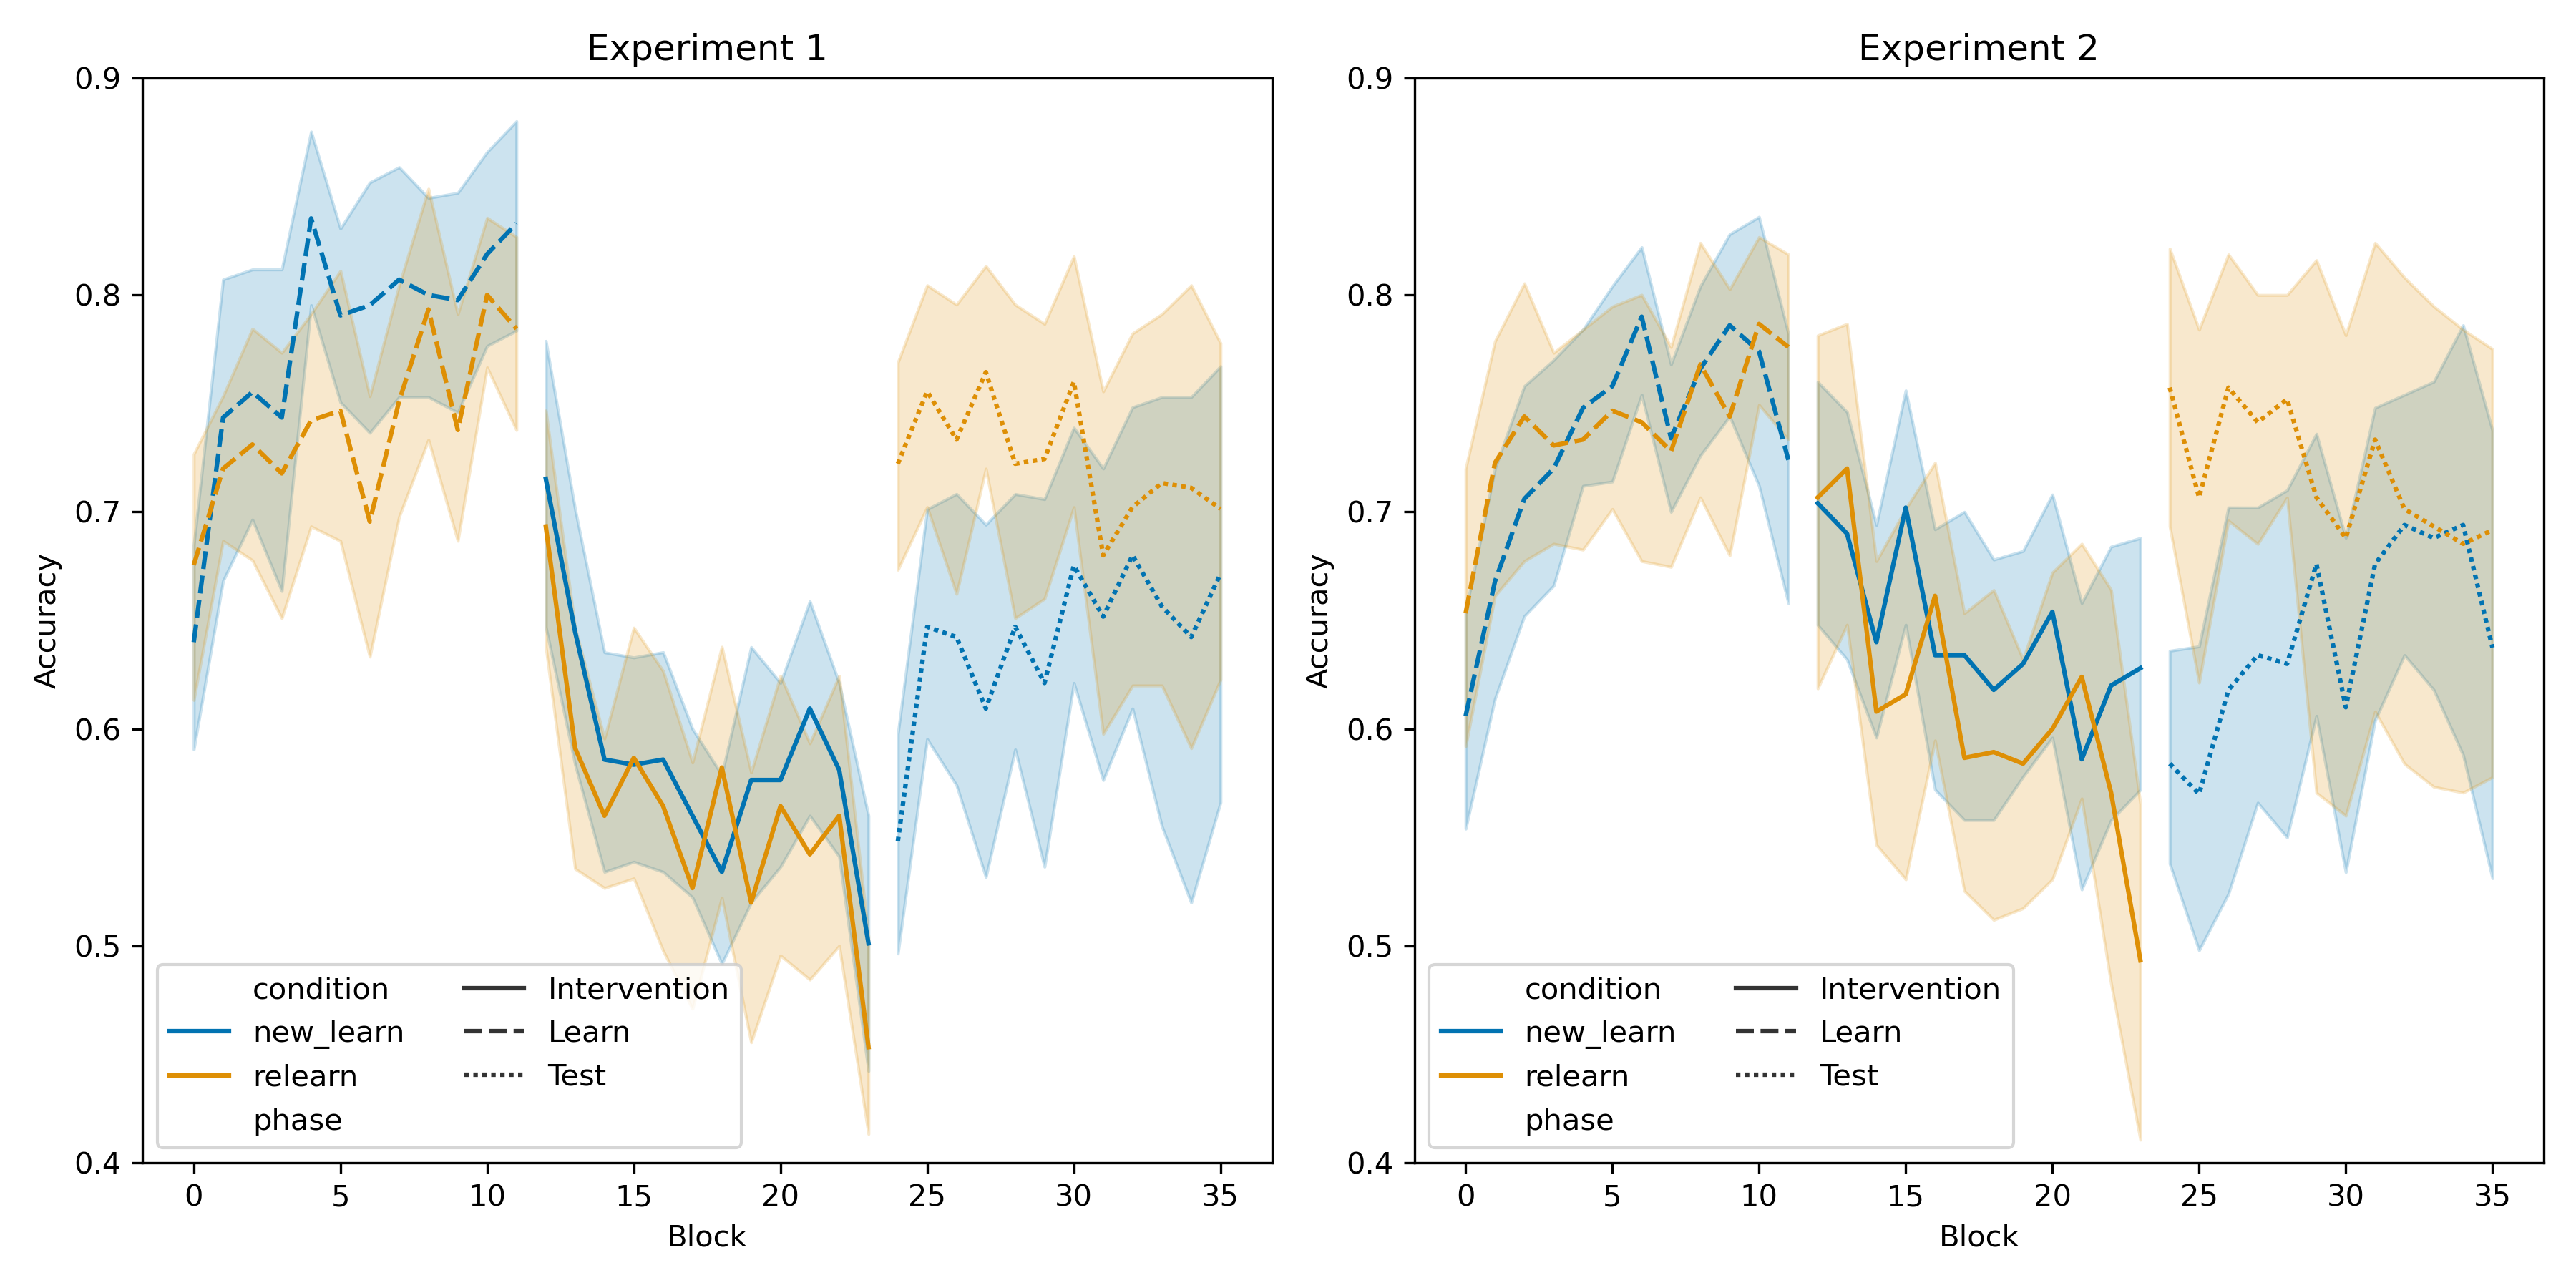
\includegraphics[width=\textwidth]{../figures/subjects_accuracy_all.png}
    \caption{
        Accuracy over blocks for all participants. Separate
        lines represent different conditions within each
        experiment.
}
\label{fig_learning_curves}
\end{figure}

Although the results suggest that the mixed-feedback
intervention leads to memory masking rather than
overwriting, it is essential to rule out potential
contamination by the declarative system (e.g., the use of
explicit rules). To address this, we fit decision-bound
models to each participant's data from the final block of
training and the first block of testing. Our primary
questions were: (1) did participants initially acquire a
procedural strategy, and (2) did they reacquire that
strategy during the Test phase? If the intervention caused
true unlearning, there should be no difference in the
proportion of participants expressing a procedural strategy
between the Relearn and New Learn conditions during the Test
phase.

Figure~\ref{fig_dbm_maps} shows heatmaps of transitions
between best-fit model classes from the end of training to
the start of testing, illustrating how participants shifted
(or failed to shift) their categorization strategies across
phases, separated by experiment and condition. In
Experiment~1, participants in the Relearn condition
predominantly acquired and reacquired a procedural strategy,
indicating that the intervention did not disrupt their
underlying category knowledge. In contrast, those in the New
Learn condition tended to switch from a procedural to a
rule-based strategy during the test phase, suggesting
interference rather than erasure. A similar pattern was
observed in Experiment~2. This further supports the
conclusion that an intervention of mixed feedback masks
rather than eliminates procedural category learning.

\begin{figure}[H]
    \centering
    \includegraphics[width=\textwidth]{../figures/best_model_class_heatmap.png}
    \caption{
        Heatmaps showing transitions between best-fit model
        classes from the end of training (Y-axis) to the
        start of testing (X-axis), separated by experiment
        and condition. Each cell indicates the number of
        participants who transitioned between model classes.
}
\label{fig_dbm_maps}
\end{figure}

Figure~\ref{fig_dbm_stats} shows Bayesian posterior
estimates of the probability that participants reacquired a
procedural strategy during the initial stages of the Test
phase. For both the Relearn and New Learn conditions, there
was little difference in reacquisition probability between
Experiment~1 and Experiment~2, as indicated by the 95\%
credible intervals that included zero (top and middle rows,
rightmost panels). However, participants in the Relearn
condition were substantially more likely to reacquire a
procedural strategy than those in the New Learn condition.
This was true in both experiments, as shown by the 95\%
credible intervals excluding zero in the bottom row's left
and middle panels. Together, these results provide strong
evidence that the intervention masked but did not erase
procedural category knowledge.

\begin{figure}[H]
    \centering
    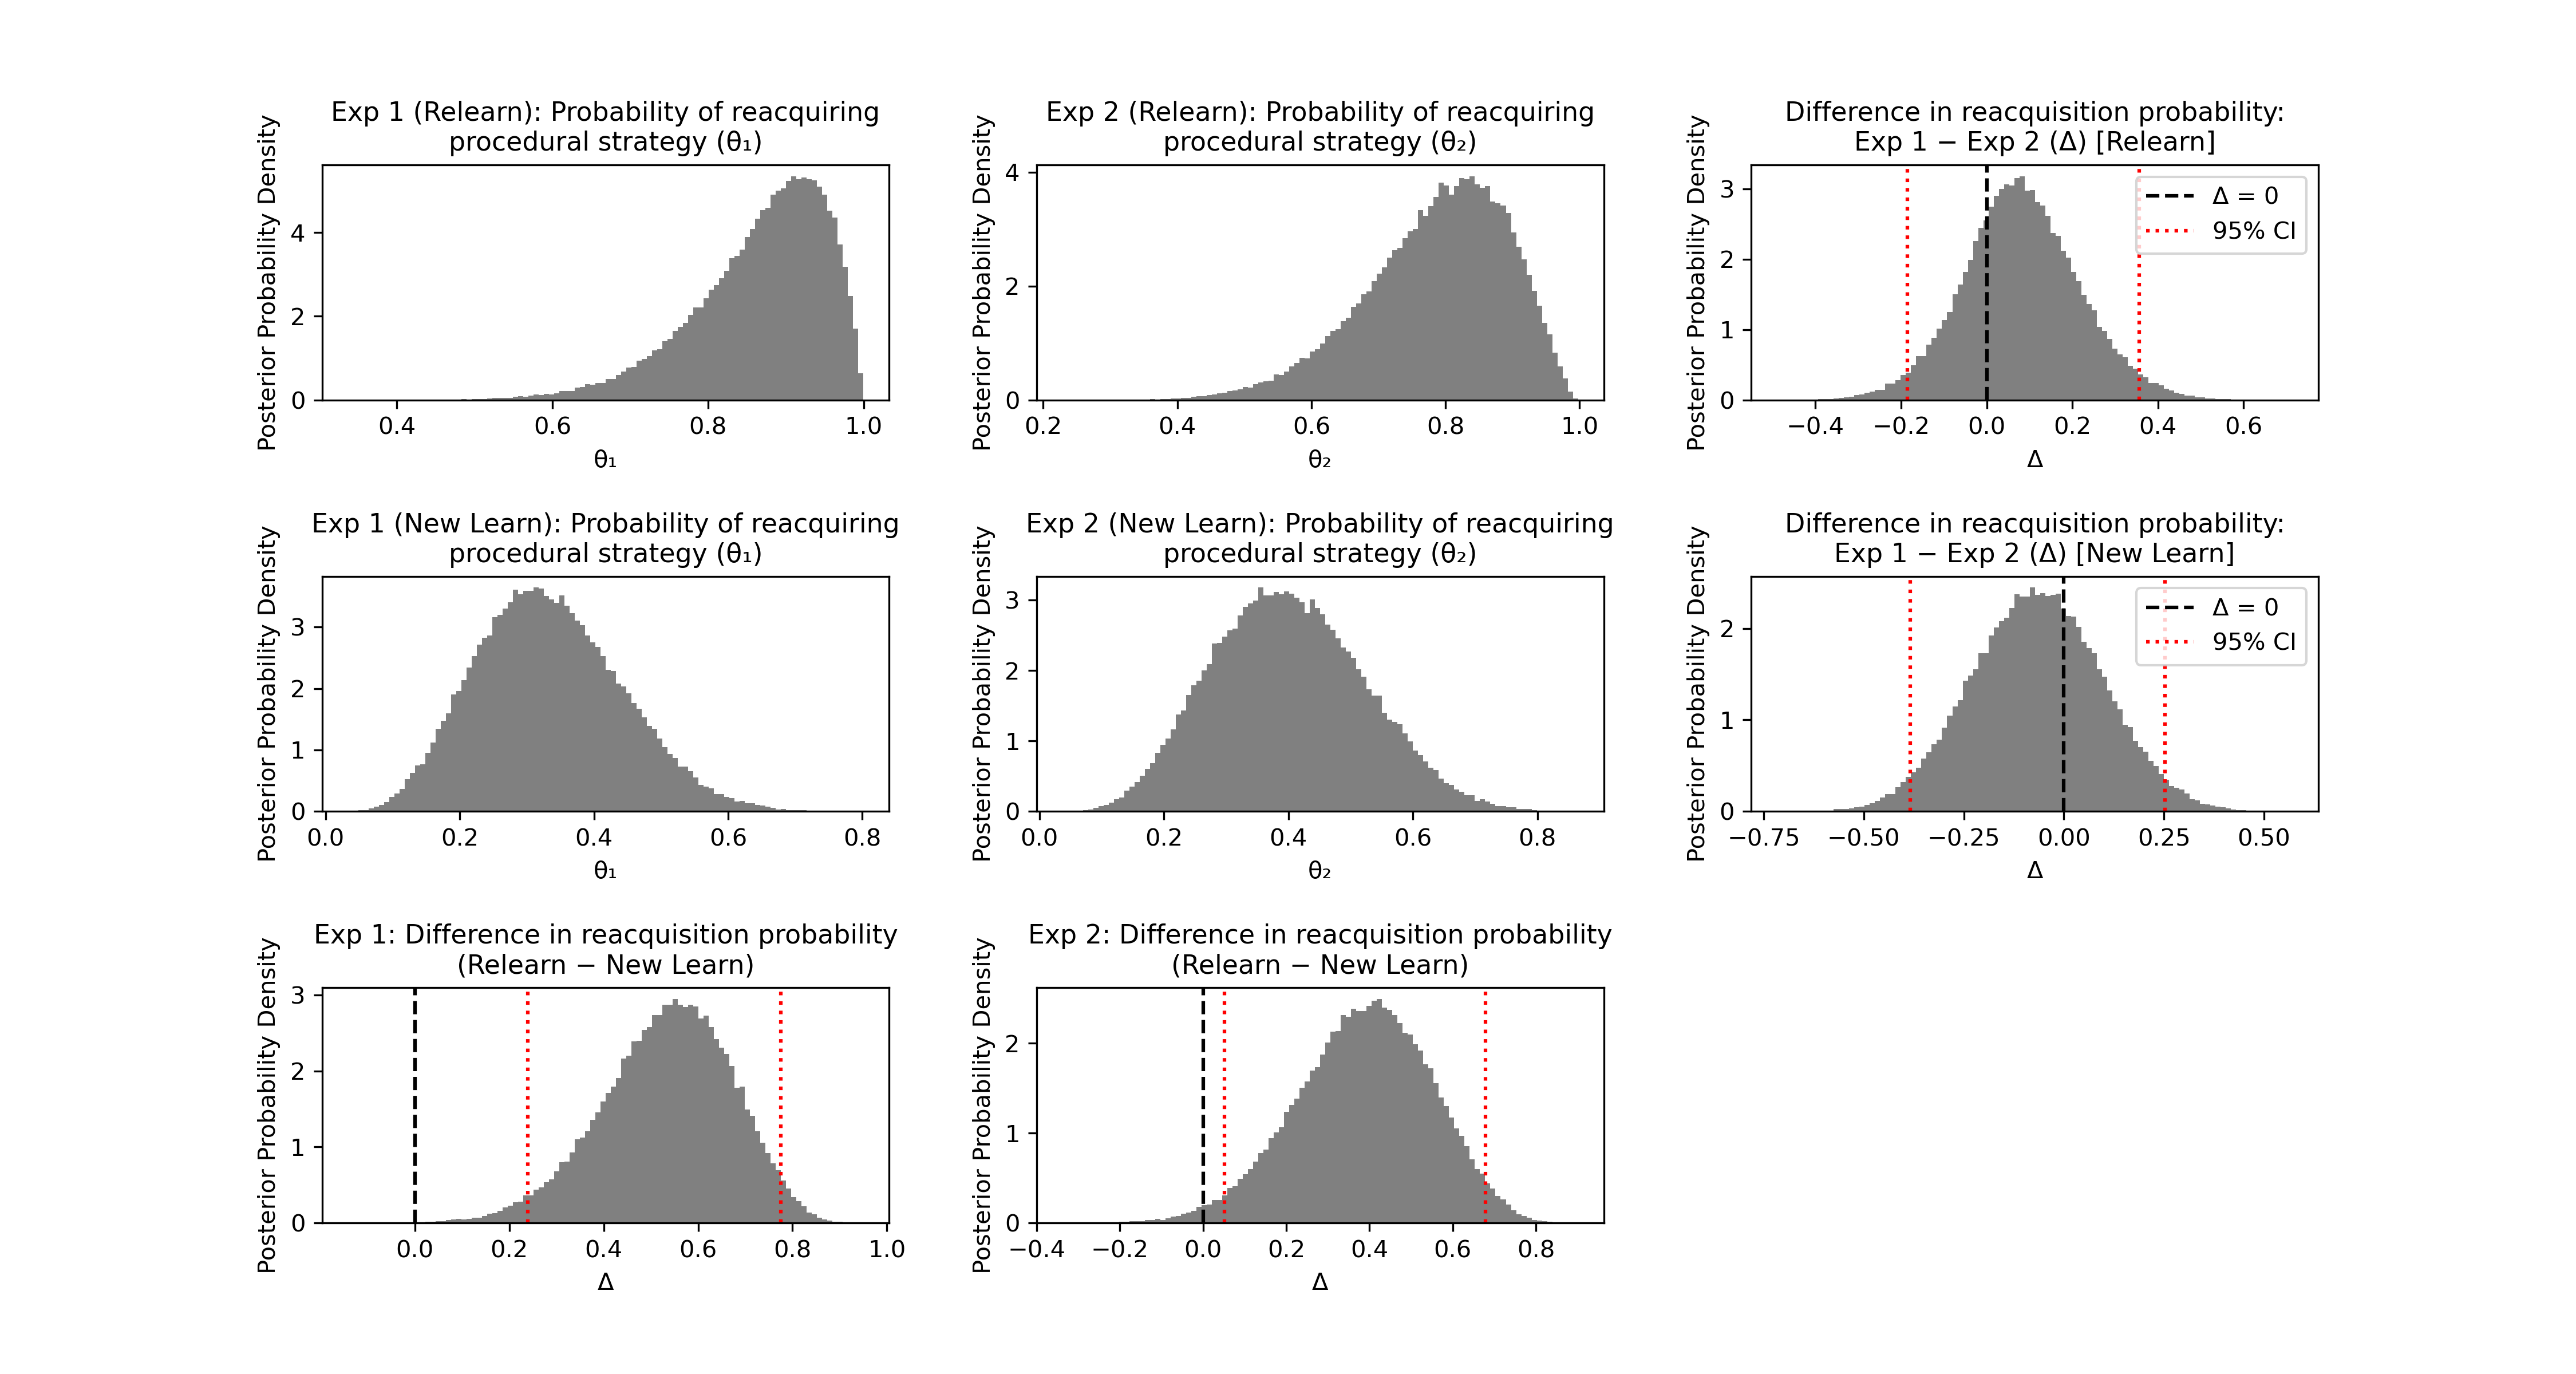
\includegraphics[width=\textwidth]{../figures/bayesian_comparison.png}
    \caption{
        Bayesian posterior distributions over $\theta$, the
        probability of reacquiring a procedural strategy.
        Top two rows show experiment comparisons within
        Relearn and New Learn conditions. Bottom row shows
        differences between conditions within each
        experiment. Red lines denote 95\% credible
        intervals; black dashed lines indicate null
        difference ($\Delta = 0$).
}
\label{fig_dbm_stats}
\end{figure}

\section{Discussion}
In previous work, mixed feedback -- where feedback about
category choices was partly random and partly veridical --
appeared to induce true unlearning of category knowledge
acquired and encoded in procedural systems.  Participants
who had acquired a category structure through procedural
learning no longer expressed evidence of this knowledge
after the intervention, consistent with the idea that the
underlying associations had been erased. An alternative
possibility, however, is that the intervention merely masked
the expression of procedural memory, leaving the underlying
stimulus-response mappings intact but temporarily dormant.
In the present study, we directly tested this possibility.
Our findings show that mixed feedback does not cause
unlearning. Instead, it masks the behavioral expression of
procedural knowledge, which remains accessible and can be
re-expressed when participants are verbally cued that valid
feedback has resumed.

\subsection{Implications for models of procedural category learning}
Ashby and Crossley (2011) and Crossley et al. (2012)
developed a biologically grounded model of how procedural
category learning is implemented in cortico-striatal basal
ganglia circuits. In this account, category knowledge is
encoded as stimulus--response associations at
cortico-striatal synapses. On its own, however, this
mechanism predicts that an intervention with purely random
feedback should overwrite the newly formed SR maps with
random associations. Our Experiment~1 results---echoing the
earlier findings of Crossley et al. (2012)---clearly show
that this does not occur. Instead, random feedback leaves
the original associations intact, implying that more is at
play than simple reinforcement learning at
cortico-striatal synapses. Specifically, there must be a
mechanism that (1) detects when feedback has become random,
and (2) protects the initial learning from modification.
Ashby and Crossley (2011) and Crossley et al. (2012)
hypothesized that this gating function is implemented by
large aspiny cholinergic interneurons in the striatum,
known as tonically active neurons (TANs). These neurons fire
tonically in their baseline state, presynaptically inhibiting
cortical input onto striatal projection neurons. When
reliable rewards are present, TANs learn to pause, thereby
permitting cortico-striatal transmission and allowing
learning. When reward contingencies break down (e.g.,
extinction or random feedback), TANs cease pausing,
shielding existing SR associations from degradation. This
gating mechanism provides a natural account of why learned
procedural knowledge can be rapidly re-expressed during the
Test phase.

Crossley et al. (2012) reported that mixed feedback appeared
to cause true unlearning. In their model, the small amount
of veridical feedback maintained the gating signal (because
contingencies were still partially reliable), leaving
cortico-striatal associations vulnerable to overwriting.
Thus, the model predicted that mixed feedback should induce
unlearning. Our current results directly contradict this
assumption. Mixed feedback did not erase procedural category
knowledge; rather, it masked its expression. This implies
that the original model requires revision. 

One alternative is that the relevant neural circuits
implement a more sophisticated mechanism that allocates,
maintains, and switches between distinct context-specific
sets of SR associations. Such an idea has been formalized in
recent mathematical models that account for a broad range of
behavioral findings \cite{gershman_context_2010}.
However, unlike our earlier work, these models are not
tightly constrained by neurobiology. Recent evidence
suggests that the TANs may in fact, support such a gating
mechanism. For example, these circuits are implicated in
tasks that require flexible switching between behavioral
policies \cite{bradfield_thalamostriatal_2018}.
Interpretation, however, remains difficult: the precise
anatomical regions examined in much of this work are often
associated with flexible cognitive control and only
ambiguously linked to SR learning \cite{yin_role_2006}.
These areas are adjacent to those highlighted in our earlier
computational and work \cite{ashby_computational_2011,
crossley_erasing_2013, crossley_context-dependent_2014,
crossley_expanding_2016}, which more directly implicate
striatal circuits in procedural SR learning.

\subsection{Broader Implications}
The present findings speak to a central issue in the study
of procedural skills and habit-like behaviors: the critical
distinction between unlearning and masking. In both animal
and human literatures, it is well recognized that the
disappearance of a behavior does not necessarily imply that
the underlying associations have been unlearned. This
distinction has important consequences for how we
conceptualize and treat maladaptive habits.

A key question is whether effective interventions must
produce true unlearning—overwriting or restructuring the
original stimulus--response associations—or whether masking
their expression may in some contexts be sufficient.
Although masking can temporarily suppress undesirable
behaviors, it leaves the underlying associations intact and
thus vulnerable to relapse once contextual cues or
contingencies change. From this perspective, masking may be
a weak or unstable intervention outcome compared with
genuine unlearning.

Our results therefore underscore the importance of clearly
distinguishing between interventions that induce unlearning
and those that merely mask behavior. This distinction is
vital not only for advancing theoretical models of
procedural learning but also for the design of practical
strategies to modify maladaptive habits in real-world
settings.

\subsection{Limitations and future directions}
One limitation of the present work concerns effective sample
size. Although the raw number of participants was adequate,
only a subset reliably acquired a procedural strategy during
the learning phase. This necessarily reduced the number of
participants available for testing our critical hypotheses.
Nevertheless, our Bayesian approach allowed us to make
strong inferences despite this reduction by quantifying
uncertainty directly and providing posterior probabilities
over key parameters.

Looking ahead, two avenues for future work are especially
important. First, the computational model developed by Ashby
and Crossley (2011) and Crossley et al. (2012) must be
revised to account for masking rather than unlearning, so
that it more accurately reflects the present findings.
Second, further experimental work is needed to identify
interventions capable of producing genuine unlearning of
procedural knowledge. Establishing such conditions would not
only clarify the boundary between masking and unlearning but
also inform the design of effective strategies for modifying
maladaptive habit-like behaviors.

\end{document}

